%--------------------------------------------CAPA DE RELACIONES------------------------------------------------------%

\subsection{Relaciones y conectores de relaciones}
% Descripción introductoria de las relaciones en ArchiMate
El lenguaje ArchiMate define un conjunto central de relaciones genéricas, cada una de las cuales puede conectar un conjunto predefinido de conceptos de origen y destino (en la mayoría de los casos, elementos, pero en algunos casos también otras relaciones). Muchas de estas relaciones están “sobrecargadas”; es decir, su significado exacto difiere según los conceptos de origen y destino que conectan. Las Tablas \ref{tab:Tabla de relaciones 1}, \ref{tab:Tabla de relaciones 2} y \ref{tab:Tabla de relaciones 3} ofrecen una descripción general de las relaciones de ArchiMate con sus definiciones. \cite{archimate} 

%---------------------------------------------------------------------------------------------------------
% TABLA 1: RELACIONES ESTRUCTURALES
%---------------------------------------------------------------------------------------------------------
\begin{longtable}{|p{0.15\linewidth}|p{0.45\linewidth}|p{0.2\linewidth}|p{0.2\linewidth}|}
    % Configuración de la caption y encabezado
    \caption{Tabla de relaciones estructurales} \label{tab:Tabla de relaciones 1} \\
    \hline
    \rowcolor[HTML]{DAE8FC} 
    \textbf{Relaciones estructurales} & \textbf{Definición} & \textbf{Notación} & \textbf{Nombres de Roles} \\
    \hline
    \endhead % Fin del encabezado repetido en cada página
    \hline
    \multicolumn{4}{r}{\textit{Continúa en la siguiente página}} \\
    \endfoot % Pie de página en páginas intermedias
    \hline
    \endlastfoot % Fin de la tabla en la última página

    % Fila 1: Composición
    Composición &
    Representa que un elemento consta de uno o más conceptos. &
    \begin{center}
        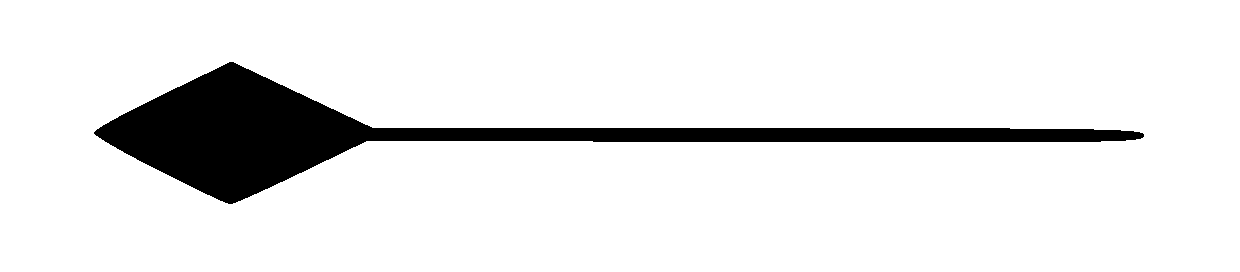
\includegraphics[width=1\linewidth]{imgs/relaciones/composicion.pdf}
    \end{center} &
    \begin{center}
        → compuesto de \\ ← compuesto en
    \end{center} \\
    \hline

    % Fila 2: Agregación
    Agregación &
    Representa que un elemento combina uno o más conceptos. &
    \begin{center}
        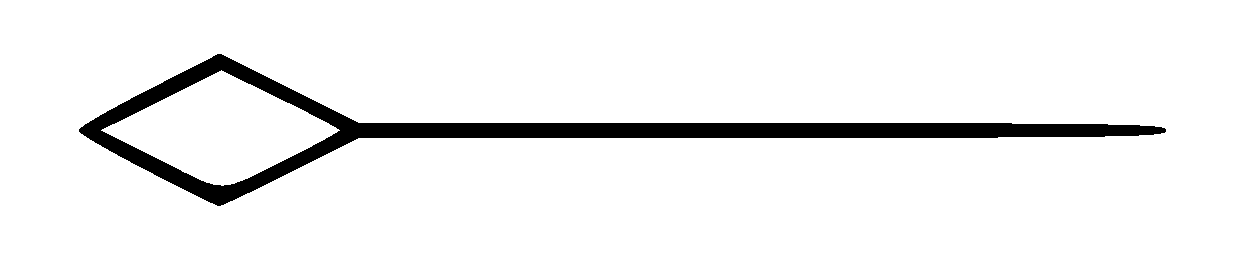
\includegraphics[width=1\linewidth]{imgs/relaciones/agregacion.pdf}
    \end{center} &
    \begin{center}
        → agregados \\ ← agregado en
    \end{center} \\
    \hline

    % Fila 3: Asignación
    Asignación &
    Representa la asignación de responsabilidad, desempeño de comportamiento, almacenamiento o ejecución. &
    \begin{center}
        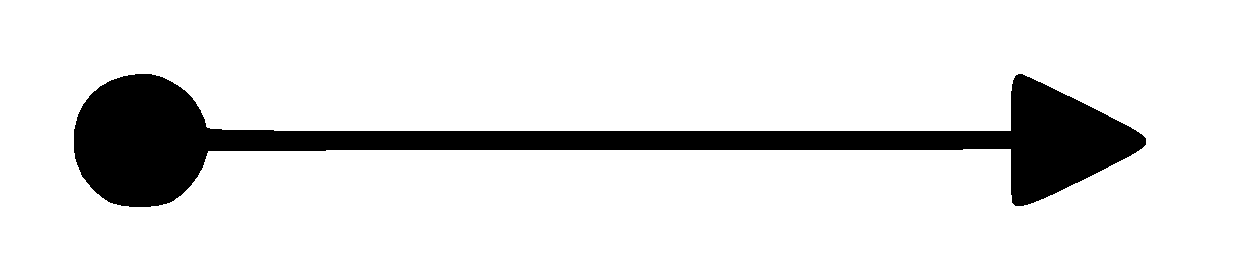
\includegraphics[width=1\linewidth]{imgs/relaciones/asignacion.pdf}
    \end{center} &
    \begin{center}
        → asignado a \\ ← ha asignado
    \end{center} \\
    \hline

    % Fila 4: Realización
    Realización &
    Representa que un elemento juega un papel crítico en la creación, logro, sustento u operación de un elemento más abstracto. &
    \begin{center}
        
\includegraphics[width=1\linewidth]{imgs/relaciones/realizacion.pdf}
    \end{center} &
    \begin{center}
        → realiza \\ ← realizado por
    \end{center} \\
    \hline
\end{longtable}

%---------------------------------------------------------------------------------------------------------
% TABLA 2: RELACIONES DE DEPENDENCIA
%---------------------------------------------------------------------------------------------------------
\begin{longtable}{|p{0.15\linewidth}|p{0.45\linewidth}|p{0.2\linewidth}|p{0.2\linewidth}|}
    % Configuración de la caption y encabezado
    \caption{Tabla de relaciones de dependencia} \label{tab:Tabla de relaciones 2} \\
    \hline
    \rowcolor[HTML]{DAE8FC} 
    \textbf{Relaciones de dependencia} & \textbf{Definición} & \textbf{Notación} & \textbf{Nombres de Roles} \\
    \hline
    \endhead % Fin del encabezado repetido en cada página
    \hline
    \multicolumn{4}{r}{\textit{Continúa en la siguiente página}} \\
    \endfoot % Pie de página en páginas intermedias
    \hline
    \endlastfoot % Fin de la tabla en la última página

    % Fila 1: Servicio
    Servicio &
    Representa que un elemento proporciona su funcionalidad a otro elemento. &
    \begin{center}
        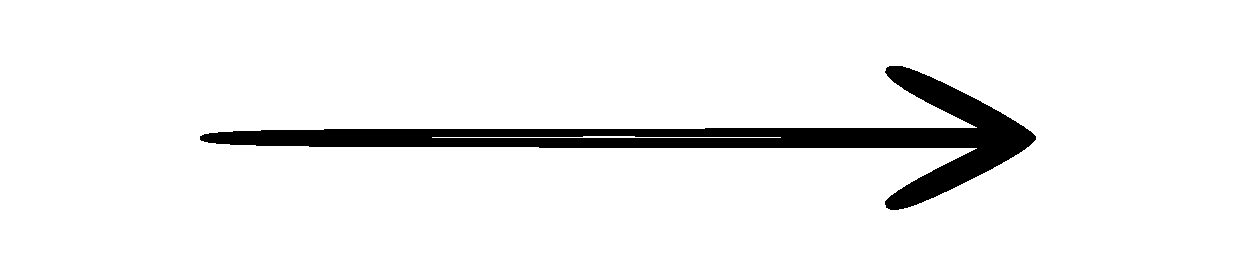
\includegraphics[width=1\linewidth]{imgs/relaciones/servicio.pdf}
    \end{center} &
    \begin{center}
        → sirve \\ ← servido por
    \end{center} \\
    \hline

    % Fila 2: Acceso
    Acceso &
    Representa la capacidad del comportamiento y de los elementos de la estructura activa para observar o actuar sobre los elementos de la estructura pasiva. &
    \begin{center}
        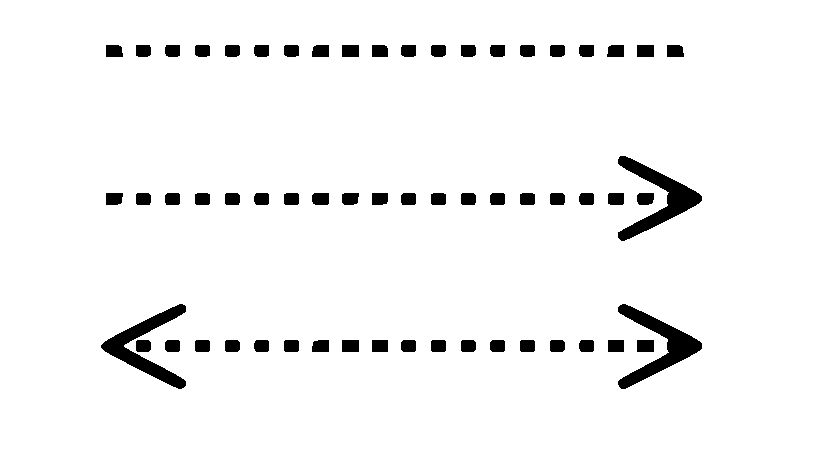
\includegraphics[width=1\linewidth]{imgs/relaciones/acceso.pdf}
    \end{center} &
    \begin{center}
        → accesos \\ ← accedido por
    \end{center} \\
    \hline

    % Fila 3: Influencia
    Influencia &
    Representa que un elemento afecta la implementación o logro de algún elemento de motivación. &
    \begin{center}
        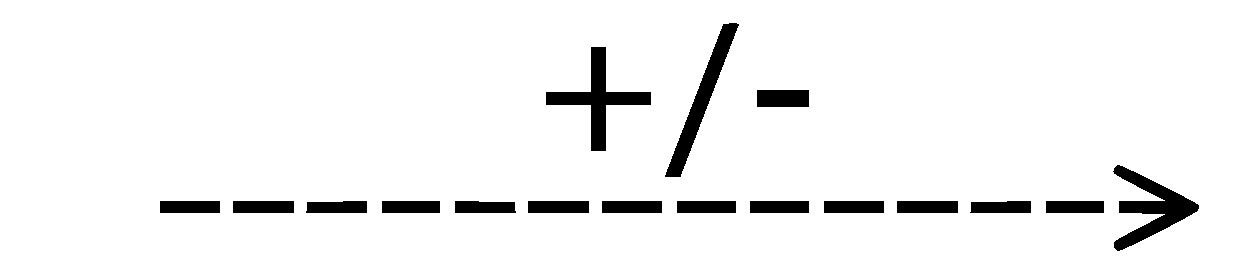
\includegraphics[width=1\linewidth]{imgs/relaciones/influencia.pdf}
    \end{center} &
    \begin{center}
        → influye \\ ← influido por % Corrección semántica para consistencia
    \end{center} \\
    \hline

    % Fila 4: Asociación
    Asociación &
    Representa una relación no especificada o una que no está representada por otra relación ArchiMate. &
    \begin{center}
        
\includegraphics[width=1\linewidth]{imgs/relaciones/asociacion.pdf}
    \end{center} &
    \begin{center}
        → asociado a \\ ← asociado de
    \end{center} \\
    \hline
\end{longtable}

%---------------------------------------------------------------------------------------------------------
% TABLA 3: CONECTORES DE RELACIONES
%---------------------------------------------------------------------------------------------------------
\begin{longtable}{|p{0.15\linewidth}|p{0.45\linewidth}|p{0.2\linewidth}|p{0.2\linewidth}|}
    % Configuración de la caption y encabezado
    \caption{Tabla de conectores de relaciones} \label{tab:Tabla de relaciones 3} \\
    \hline
    \rowcolor[HTML]{DAE8FC} 
    \textbf{Conectores de relación} & \textbf{Definición} & \textbf{Notación} & \textbf{Nombres de Roles} \\
    \hline
    \endhead % Fin del encabezado repetido en cada página
    \hline
    \multicolumn{4}{r}{\textit{Continúa en la siguiente página}} \\
    \endfoot % Pie de página en páginas intermedias
    \hline
    \endlastfoot % Fin de la tabla en la última página

    % Fila 1: Unión
    Unión &
    Se utiliza para conectar relaciones del mismo tipo. &
    \begin{center}
        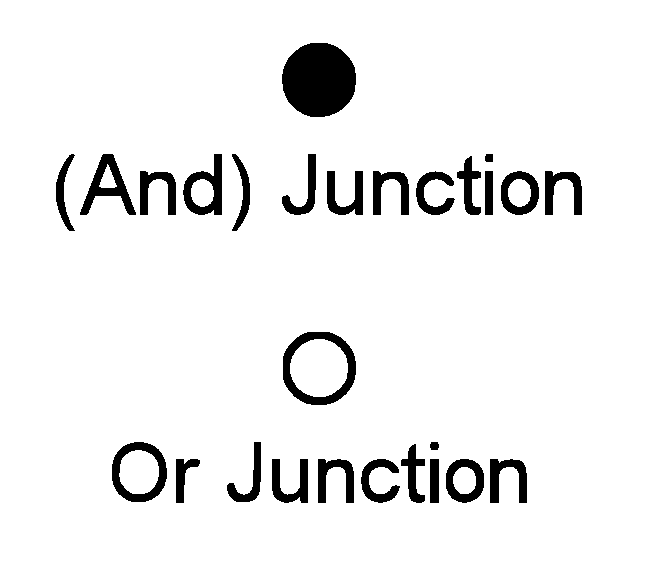
\includegraphics[width=1\linewidth]{imgs/relaciones/union.pdf}
    \end{center} &
    \begin{center}
        → asociado a \\ ← asociado de
    \end{center} \\
    \hline
\end{longtable}